\chapter{SmartScan}

SmartScan is a desktop application that aims to help begginer developers evaluate their projects from a security standpoint while it can also help regular users evaluate how safe a smart contract is. The main purpose of this project is to be easy to use, but also powerful enough to provide relevant insight and guidance towards fixing the security vulnerabilities. For this purpose, SmartScan uses the GitHub REST API \cite{gitHubRestAPI} for a quick and intuitive project cloning process and Slither \cite{slitherGitHub} for the analysis of the cloned project.

The choice for the analysis tool was not difficult for multiple reasons, as conveyed by the previous chapter. The first one is in its core design: being a static analysis tool makes it great for scanning projects without executing them, which would have added complexity to the entire setup. Secondly, its balance between high performance and low execution time in terms of scanning for security threats is great for providing fast and reliable vulnerability reports.

\begin{figure}[h]
    \centering
    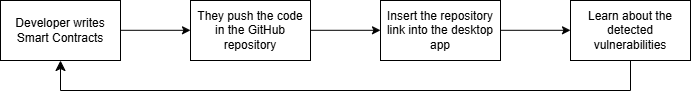
\includegraphics[width=1\linewidth]{images/scenario-diagram.png}
    \caption{Scenario diagram for SmartScan.}
    \label{fig:enter-label}
\end{figure}

As shown in the diagram above, the usual workflow in which SmartScan is involved starts with the developer writing the smart contract code and pushing it in the GitHub repository. Out application intervenes right after, when the developer copies the repository link in it and starts the analysis. Afterwards, the application returns a security report, based on which the developer may start fixing the vulnerabilities and the cycle may repeat. Whenever the application runs the analysis, it makes sure to fetch the latest version of the project so the developer doesn't need to.

\begin{figure}[h]
    \centering
    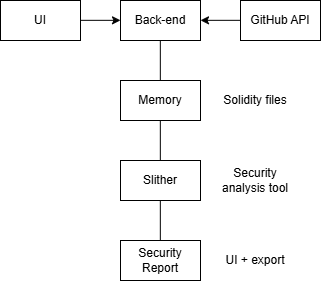
\includegraphics[width=0.5\linewidth]{images/component-diagram.png}
    \caption{Component diagram for SmartScan.}
    \label{fig:enter-label}
\end{figure}

In terms of infrastructure and design choices, SmartScan is developed in Python, using the PySide 6 framework \cite{pySide6} for the interface because it provides a clean and easy to use design with minimal performance limitations. The back-end of the application consists of the aforementioned REST API and Slither, linked together with custom scripts designed to manage the analysis results.

\begin{figure}[h]
    \centering
    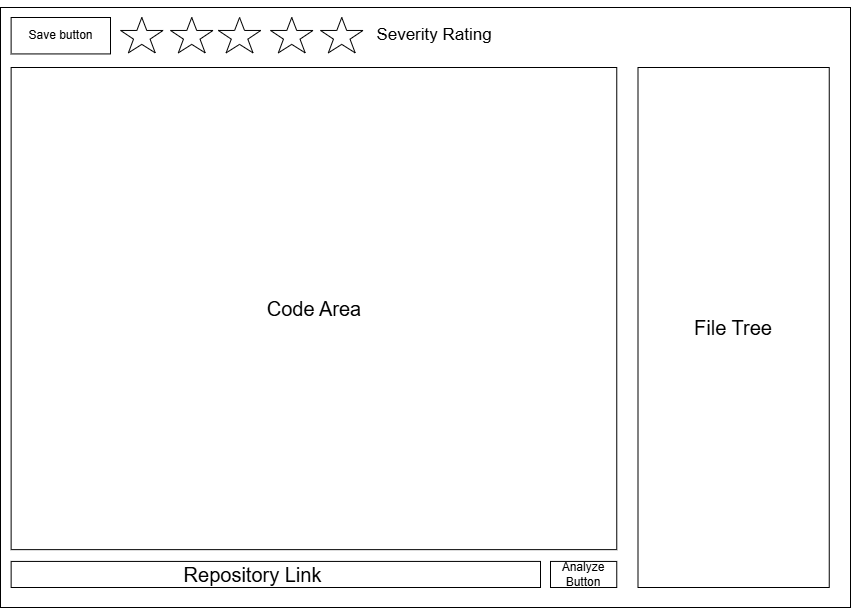
\includegraphics[width=0.80\linewidth]{images/application-design.png}
    \caption{SmartScan's User Interface.}
    \label{fig:enter-label}
\end{figure}

The figure above presents the user interface of SmartScan. The first component the user will interact with is the Repository Link text box, in which they will insert the repository link copied from GitHub before pressing the Analyze Button. Afterwards, the REST API will handle the cloning of the project and Slither will analyze it, returning all the found vulnerabilities. The File Tree is used to access the cloned project and open any Solidity file in order to see the code inside. The Code Area will host the code of the currently open file, with a side bar that shows the number of each line and a yellow highlight that shows which lines of code are vulnerable, as detected by Slither. The side bar and the highlight are meant to visually guide the developer towards the problem with ease. After fixing the code, the user may save the file through the dedicated button on the top left corner.

SmartScan, while using external APIs for cloning and analyzing the project, compiles a security report of its own, based on the vulnerabilities found by Slither. The whole report will be saved in a separate text file, so the user can access it whenever they want, and will be shown in the Code Area at the end of the analysis. Also, the stars next to the Save Button will turn red depending on the determined severity of the project. The metric used to measure how vulnerable a project is will be the amount of threats found and their severity. Each star turning red represents a higher vulnerability of the project as a whole. Ideally, the analyzed project should get a rating of zero stars, while a five-star rating is the worst case possible.

\begin{table}[h]
\centering
\begin{tabular}{|c|c|}
\hline
Star rating & Condition                                                              \\ \hline
0 $\star$   & No vulnerability found                                                 \\ \hline
1 $\star$   & $\leq 10$ vulnerabilities, no high severity ones                       \\ \hline
2 $\star$   & $\leq 25$ vulnerabilities, $\leq 2$ of high severity, no critical ones \\ \hline
3 $\star$   & $> 25$ vulnerabilities, $\leq 5$ of high severity, no critical ones    \\ \hline
4 $\star$   & $\leq 10$ high vulnerabilities or $\leq 2$ critical ones               \\ \hline
5 $\star$   & $> 10$ high vulnerabilities or $> 2$ critical ones                     \\ \hline
\end{tabular}
\caption{Project vulnerability rating done by SmartCheck.}
\label{tab:my-table}
\end{table}

A zero-star rating is obtained if Slither finds no security issue (informational and optimization issues are not included). A One-star rating is awarded if Slither finds less than 10 vulnerabilities, none of which are of high or critical severity. For a project to get a three-star rating, the project is required to have no critical vulnerability, but is allowed to have up to five high severity vulnerabilities. If any critical vulnerability is found, the project will get a rating of four or five stars regardless of how many issues are found.

The idea behind this rating is to raise awareness to the developer towards the security threats and induce a sense of urgency towards solving the high and critical vulnerabilities. For this reason, any critical vulnerability found will grant a minimum of four stars, while projects with no high severity vulnerabilities will only get one star. Furthermode, while one could argue that the rating should factor in the project's complexity and allow more vulnerabilities for larger projects, we should also consider that high-scale projects may also get targeted more often by attackers while the financial stakes are also higher. As such, the state of a project's security should not be influenced by its size.


\begin{figure}[h]
    \centering
    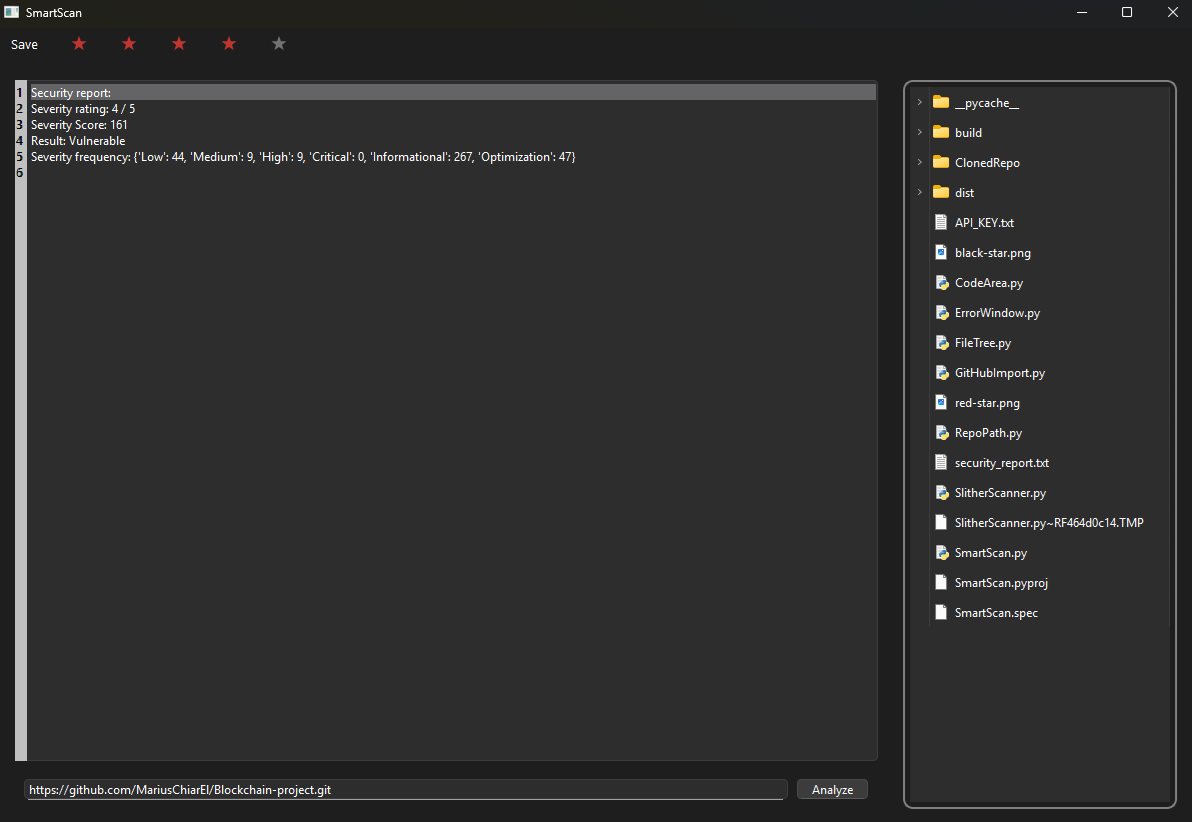
\includegraphics[width=1\linewidth]{images/application-design-in-practice.png}
    \caption{SmartScan's User Interface in practice: The Code Area features the final security report of a smart contract.}
    \label{fig:enter-label}
\end{figure}

As shown in the screenshot above, our sample smart contract project obtained a rating of four stars. Despite having no critical security issue, the high severity vulnerabilities are the root cause of these results. In this project, Slither had found 44 low severity errors, nine of medium severity and another nine of high severity. Additionally, the tool found 47 opportunities to optimize the smart contract and 267 informational errors, which are often not indicating any direct problems for the end user.

\begin{figure}[h]
    \centering
    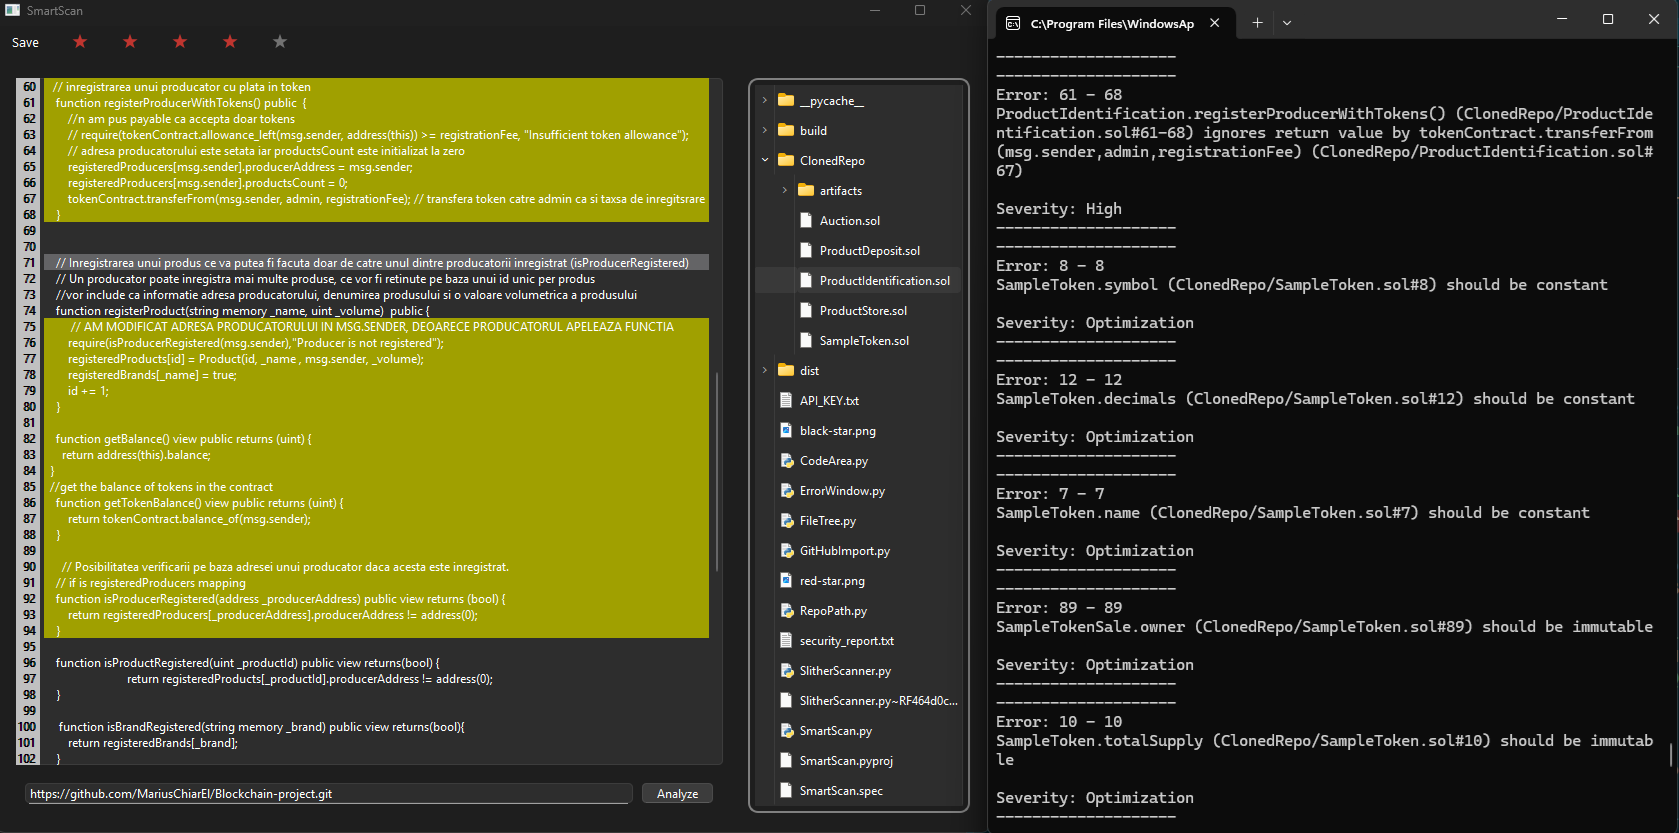
\includegraphics[width=1\linewidth]{images/highlighted-errors.png}
    \caption{SmartScan's User Interface in practice: The Code Area features the code of a Solidity file with its affected lines highlighted. The console shows the description of each error.}
    \label{fig:enter-label}
\end{figure}

In this figure we can see SmartScan in action, highlighting the affected code, as reported in the console
%[Show the final reports for various projects]

%[IDEA: SmartScan can generate a text report of all the errors for the developer to track]
%[IDEA: SmartScan can be used by students to pinpoint the security flaws in their projects (educational use case)]

%[Future work / Good to have additions: highlight different severity vulnerabilities with different colors (gradient from yellow to red), use git.diff, separate window that shows the error in the affected code under the cursor, making it a web application]